\documentclass[11pt,a4paper]{article}
\usepackage[utf8]{inputenc}
\usepackage{amsmath,amsfonts,amssymb}
\usepackage{graphicx}
\usepackage{geometry}
\geometry{top=0.65in,bottom=0.65in,left=0.75in,right=0.75in}
\usepackage{booktabs}
\usepackage{hyperref}
\usepackage{float}
\usepackage{xcolor}

\definecolor{darkbg}{HTML}{0d121f}
\definecolor{lighttext}{HTML}{e2e8f0}
\definecolor{primary}{HTML}{8b5cf6}
\definecolor{secondary}{HTML}{0dd5c5}
\definecolor{accent}{HTML}{10b981}

\pagecolor{darkbg}
\color{lighttext}

\hypersetup{
    colorlinks=true,
    linkcolor=secondary,
    urlcolor=secondary,
    citecolor=accent
}

\title{\textbf{EE3621: Digital Signal Processing} \\ \Large Student Lecture Notes — Lecture 25 \\ \large Design of IIR Filters — Bilinear Transformation \& Matched Z-Transform}
\author{III B.Tech EEE — Core Exam Preparation Guide}
\date{}

\begin{document}

\maketitle

\noindent\rule{\textwidth}{0.5pt}

\section{Core Concept of the Bilinear Transformation (BLT)}

\subsection{Derivation from the Trapezoidal Integration Rule}
The \textbf{Bilinear Transformation (BLT)} is an algebraic mapping derived by approximating continuous integration via numerical trapezoidal integration. Consider an ideal analog integrator:
\begin{equation}
H_a(s) = \frac{Y(s)}{X(s)} = \frac{1}{s} \iff \frac{dy(t)}{dt} = x(t)
\end{equation}
Integrating both sides between the sampling instants $t = (n-1)T$ and $t = nT$:
\begin{equation}
y(nT) - y((n-1)T) = \int_{(n-1)T}^{nT} x(t) \, dt
\end{equation}
Applying the \textbf{trapezoidal rule} to approximate the area under the curve:
\begin{equation}
\int_{(n-1)T}^{nT} x(t) \, dt \approx \frac{T}{2} [x(nT) + x((n-1)T)]
\end{equation}
Substituting this into the discrete difference equation ($y[n] \equiv y(nT)$):
\begin{equation}
y[n] - y[n-1] = \frac{T}{2} [x[n] + x[n-1]]
\end{equation}
Taking the $Z$-transform on both sides:
\begin{align}
Y(z) - z^{-1} Y(z) &= \frac{T}{2} [X(z) + z^{-1} X(z)] \nonumber \\
Y(z)(1 - z^{-1}) &= \frac{T}{2} X(z)(1 + z^{-1}) \implies H(z) = \frac{Y(z)}{X(z)} = \frac{T}{2} \left(\frac{1 + z^{-1}}{1 - z^{-1}}\right)
\end{align}
Equating the analog integrator $H_a(s) = \frac{1}{s}$ to the discrete integrator $H(z)$:
\begin{equation}
\frac{1}{s} = \frac{T}{2} \left(\frac{1 + z^{-1}}{1 - z^{-1}}\right) \implies \mathbf{s = \frac{2}{T} \left( \frac{1 - z^{-1}}{1 + z^{-1}} \right) = \frac{2}{T} \left( \frac{z - 1}{z + 1} \right)}
\label{eq:blt_formula}
\end{equation}
This is the celebrated \textbf{Bilinear Transformation substitution rule}.

\subsection{Stability \& The Elimination of Aliasing}
\begin{itemize}
    \item \textbf{Guaranteed Stability:} The entire open left-half of the $s$-plane ($\text{Re}(s) < 0$) maps strictly to the interior of the unit circle ($|z| < 1$). Stable analog filters \textbf{always produce stable digital filters}.
    \item \textbf{Zero Aliasing:} The entire continuous imaginary axis $s = j\Omega$ from $-\infty$ to $+\infty$ maps **one-to-one** onto the discrete unit circle $z = e^{j\omega}$ from $-\pi$ to $+\pi$.
    \item \textbf{Universal Applicability:} Because there is no aliasing, BLT can design **Lowpass, Highpass, Bandpass, and Bandstop filters**!
\end{itemize}

\begin{figure}[H]
\centering
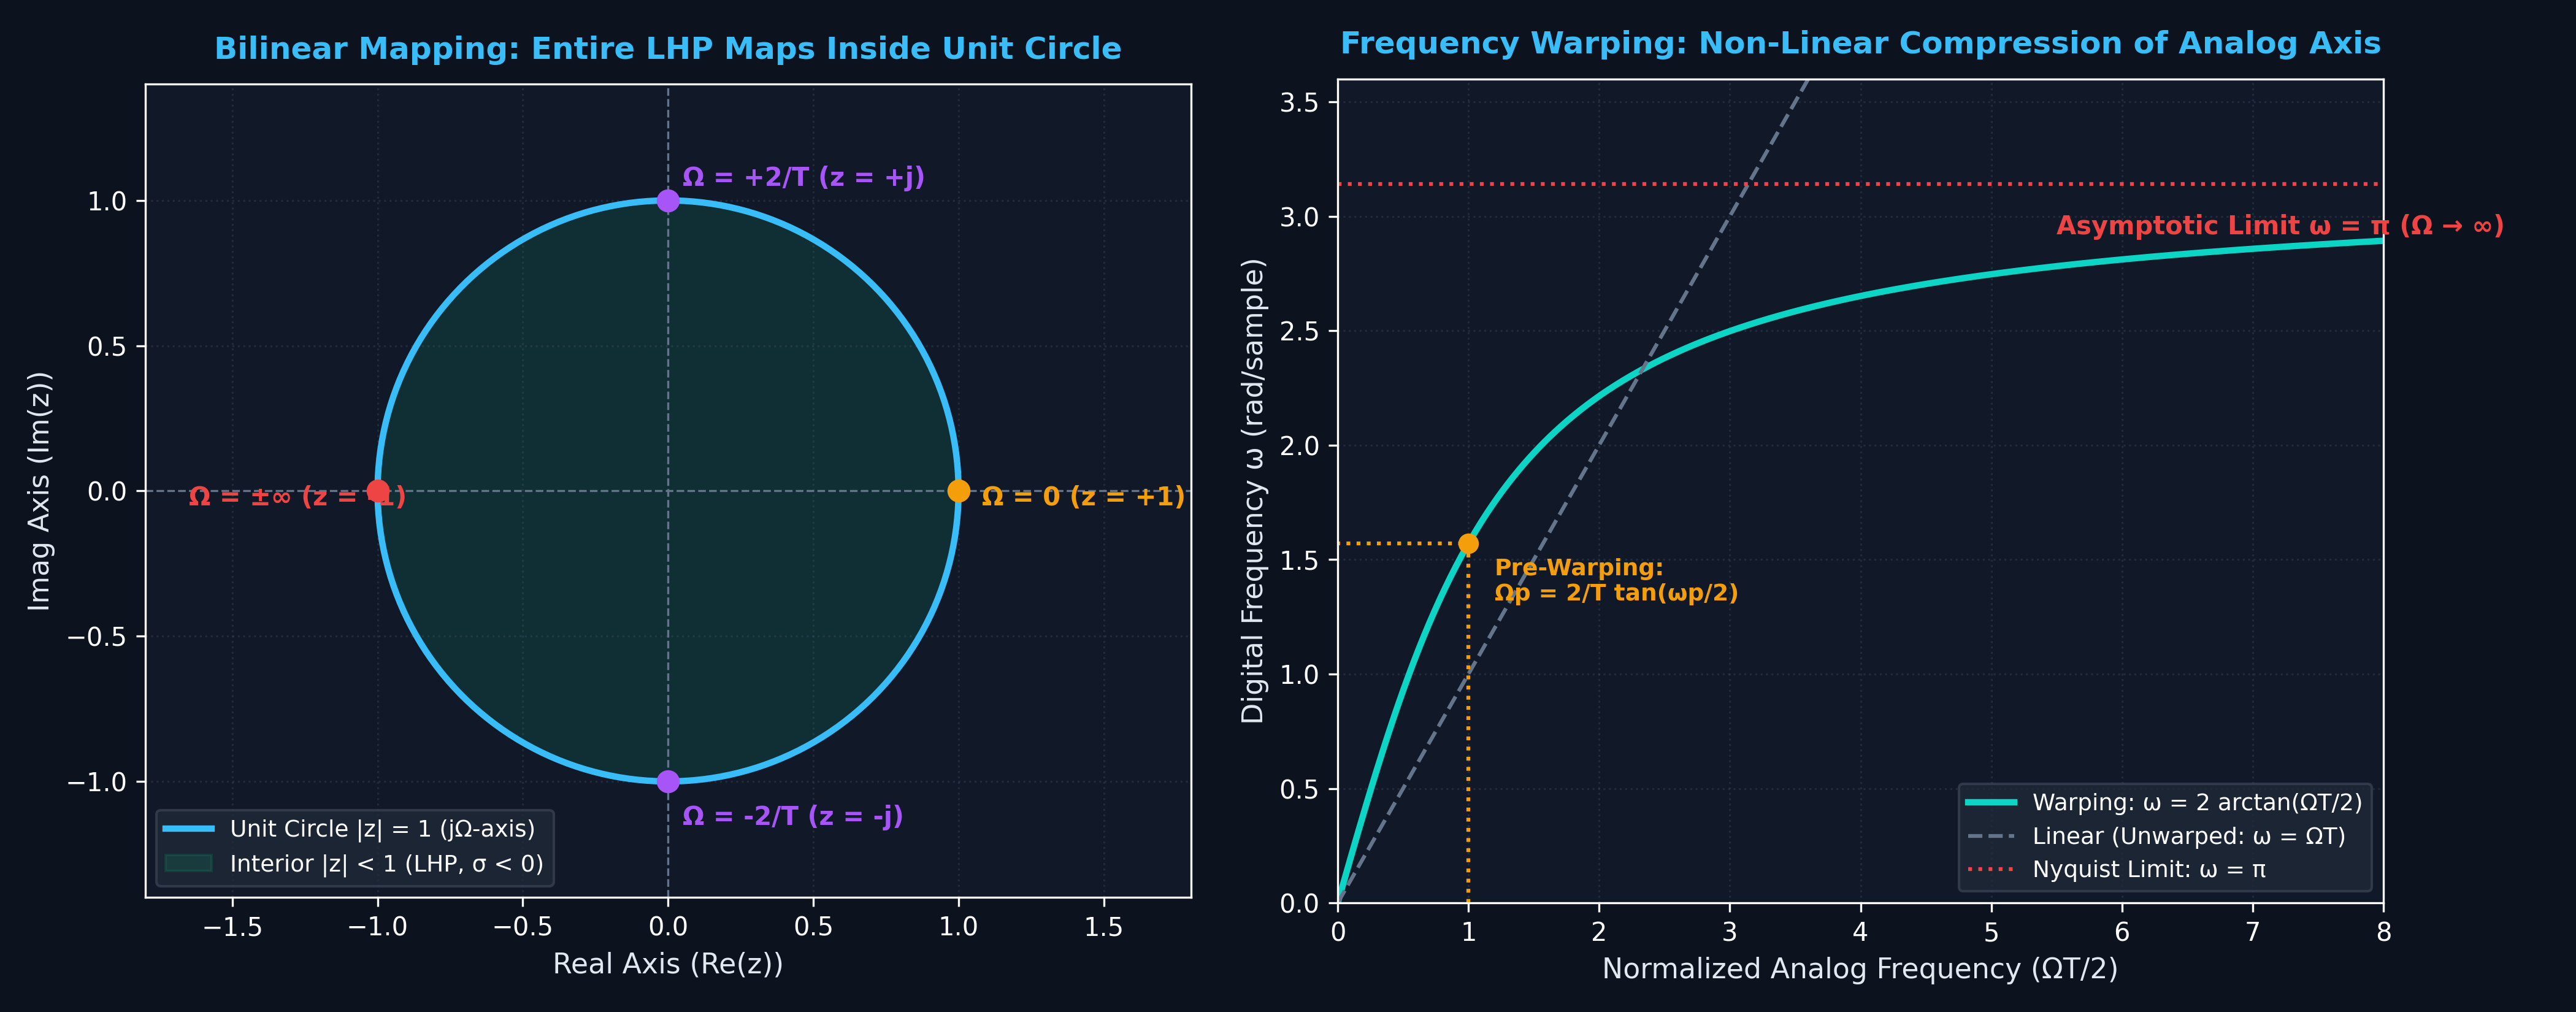
\includegraphics[width=0.55\textwidth]{images/iir_bilinear_transform_warping.png}
\caption{Left: One-to-one mapping from $s$-plane to $z$-plane. Right: Non-linear frequency warping curve showing compression into the digital interval $[0, \pi]$.}
\label{fig:blt_summary}
\end{figure}

\noindent\rule{\textwidth}{0.5pt}

\section{Frequency Warping \& Mandatory Pre-Warping}

\subsection{Step-by-Step Derivation of the Frequency Warping Equation}
To find the relationship between analog frequency $\Omega$ and digital frequency $\omega$, evaluate the BLT substitution \eqref{eq:blt_formula} on the unit circle $z = e^{j\omega}$ ($s = j\Omega$):
\begin{align}
j\Omega &= \frac{2}{T} \left( \frac{1 - e^{-j\omega}}{1 + e^{-j\omega}} \right) = \frac{2}{T} \left[ \frac{e^{-j\omega/2} (e^{j\omega/2} - e^{-j\omega/2})}{e^{-j\omega/2} (e^{j\omega/2} + e^{-j\omega/2})} \right] \nonumber \\
&= \frac{2}{T} \left( \frac{e^{j\omega/2} - e^{-j\omega/2}}{e^{j\omega/2} + e^{-j\omega/2}} \right)
\end{align}
Using Euler's identities $e^{j\theta} - e^{-j\theta} = 2j\sin\theta$ and $e^{j\theta} + e^{-j\theta} = 2\cos\theta$:
\begin{equation}
j\Omega = \frac{2}{T} \left[ \frac{2j\sin(\omega/2)}{2\cos(\omega/2)} \right] = j \frac{2}{T} \tan\left(\frac{\omega}{2}\right)
\end{equation}
Equating imaginary parts yields the fundamental \textbf{Frequency Warping Equation}:
\begin{equation}
\mathbf{\Omega = \frac{2}{T} \tan\left(\frac{\omega}{2}\right)} \iff \mathbf{\omega = 2 \arctan\left(\frac{\Omega T}{2}\right)}
\end{equation}
The entire infinite analog axis $\Omega \in [0, \infty)$ is non-linearly compressed into the finite digital interval $\omega \in [0, \pi)$.

\subsection{The Mandatory Pre-Warping Rule}
Because frequency warping non-linearly shifts transition edges, any design specification given in digital frequencies $\omega_p, \omega_s$ \textbf{must be pre-warped} into analog frequencies before designing the analog prototype filter:
\begin{equation}
\mathbf{\Omega_p = \frac{2}{T} \tan\left(\frac{\omega_p}{2}\right)}, \qquad \mathbf{\Omega_s = \frac{2}{T} \tan\left(\frac{\omega_s}{2}\right)}
\end{equation}

\noindent\rule{\textwidth}{0.5pt}

\section{The Matched Z-Transform (MZT) Method}

The \textbf{Matched Z-Transform} maps poles and zeros individually via direct exponential substitution:
\begin{equation}
\mathbf{(s - s_k) \quad \longrightarrow \quad (1 - e^{s_k T} z^{-1})}
\end{equation}
\begin{itemize}
    \item \textbf{Poles:} $s = p_k \implies z_k = e^{p_k T}$.
    \item \textbf{Zeros at Infinity:} For an all-pole analog filter with $N$ poles and no finite zeros, add $(1 + z^{-1})$ factors in the numerator to ensure transmission nulls at Nyquist ($\omega = \pi$, $z = -1$):
    \begin{equation}
    H(z) = K_d \frac{(1 + z^{-1})^M}{\prod_{k=1}^N (1 - e^{p_k T} z^{-1})}
    \end{equation}
    \item \textbf{Gain Constant $K_d$:} Evaluated to match DC gain: $H(1) = H_a(0)$.
\end{itemize}

\noindent\rule{\textwidth}{0.5pt}

\section{Master Comparison Table of IIR Design Methods}

\begin{table}[H]
\centering
\caption{Comparison of Impulse Invariance, Bilinear Transformation, and Matched Z-Transform}
\label{tab:comp}
\vspace{2mm}
\resizebox{\textwidth}{!}{
\begin{tabular}{lccc}
\toprule
\textbf{Feature} & \textbf{Impulse Invariance} & \textbf{Bilinear Transformation (BLT)} & \textbf{Matched Z-Transform (MZT)} \\
\midrule
\textbf{Substitution Rule} & Partial fractions: $\frac{A}{s-s_k} \to \frac{T A}{1 - e^{s_k T} z^{-1}}$ & $s = \frac{2}{T}\left(\frac{1 - z^{-1}}{1 + z^{-1}}\right)$ into $H_a(s)$ & $(s - a) \to (1 - e^{a T} z^{-1})$ \\
\textbf{Aliasing} & **Severe aliasing** & **Zero aliasing** & Mild aliasing \\
\textbf{Pre-Warping} & Not applicable & **Mandatory** ($\Omega = \frac{2}{T}\tan(\omega/2)$) & Not applicable \\
\textbf{Filter Types} & LPF and BPF only (No HPF/BSF) & **Universal (LPF, HPF, BPF, BSF)** & LPF and BPF primarily \\
\textbf{Stability} & Strictly preserved & Strictly preserved & Strictly preserved \\
\bottomrule
\end{tabular}
}
\end{table}

\noindent\rule{\textwidth}{0.5pt}

\section{Standard Solved Exam Examples}

\subsection*{Solved Exam Example 1: 2nd-Order Butterworth Lowpass Filter via BLT}

\textbf{Problem 1:} Design a 2nd-order digital Butterworth lowpass filter with a 3-dB cutoff frequency $\omega_c = 0.2\pi$ rad/sample using the Bilinear Transformation with sampling interval $T = 1$ second.

\vspace{1mm}
\noindent\textbf{Solution:}

\noindent\textbf{Step 1: Pre-Warp the Digital Cutoff Frequency}
Using the fundamental pre-warping relation:
\begin{align}
\Omega_c &= \frac{2}{T} \tan\left(\frac{\omega_c}{2}\right) = \frac{2}{1} \tan\left(\frac{0.2\pi}{2}\right) = 2 \tan(0.1\pi) = 2 \tan(18^\circ) \nonumber \\
&= 2 \times 0.32492 = \mathbf{0.6498 \text{ rad/s}}
\end{align}

\noindent\textbf{Step 2: Construct the Analog Prototype Transfer Function}
A normalized 2nd-order Butterworth lowpass filter has denominator $s^2 + \sqrt{2}s + 1$. Scaling by the pre-warped cutoff $\Omega_c = 0.6498$:
\begin{equation}
H_a(s) = \frac{\Omega_c^2}{s^2 + \sqrt{2}\Omega_c s + \Omega_c^2}
\end{equation}
Evaluating coefficients with all intermediate arithmetic:
\begin{align}
\Omega_c^2 &= (0.64984)^2 = \mathbf{0.4223} \nonumber \\
\sqrt{2}\Omega_c &= 1.41421 \times 0.64984 = \mathbf{0.9190} \nonumber \\
H_a(s) &= \frac{0.4223}{s^2 + 0.9190 s + 0.4223}
\end{align}

\noindent\textbf{Step 3: Substitute the Bilinear Transformation ($T = 1$ s)}
Substitute $s = \frac{2}{T}\left(\frac{1 - z^{-1}}{1 + z^{-1}}\right) = 2\left(\frac{1 - z^{-1}}{1 + z^{-1}}\right)$:
\begin{equation}
H(z) = \frac{0.4223}{\left[2\left(\frac{1 - z^{-1}}{1 + z^{-1}}\right)\right]^2 + 0.9190\left[2\left(\frac{1 - z^{-1}}{1 + z^{-1}}\right)\right] + 0.4223}
\end{equation}
Multiply the numerator and denominator by the common denominator $(1 + z^{-1})^2$:
\begin{align}
\text{Numerator} &= 0.4223 (1 + z^{-1})^2 = \mathbf{0.4223 (1 + 2z^{-1} + z^{-2})} \nonumber \\
\text{Denominator} &= 4(1 - z^{-1})^2 + 1.8380(1 - z^{-1})(1 + z^{-1}) + 0.4223(1 + z^{-1})^2 \nonumber \\
&= 4(1 - 2z^{-1} + z^{-2}) + 1.8380(1 - z^{-2}) + 0.4223(1 + 2z^{-1} + z^{-2})
\end{align}
Collecting like powers of $z^{-1}$ step-by-step:
\begin{align}
\text{Constant ($z^0$)} &= 4(1) + 1.8380(1) + 0.4223(1) = 4 + 1.8380 + 0.4223 = \mathbf{6.2603} \nonumber \\
\text{Coefficient of $z^{-1}$} &= 4(-2) + 1.8380(0) + 0.4223(2) = -8 + 0.8446 = \mathbf{-7.1554} \nonumber \\
\text{Coefficient of $z^{-2}$} &= 4(1) + 1.8380(-1) + 0.4223(1) = 4 - 1.8380 + 0.4223 = \mathbf{2.5843}
\end{align}
The denominator is $D(z) = 6.2603 - 7.1554 z^{-1} + 2.5843 z^{-2}$. Divide all numerator and denominator terms by $6.2603$ to make the denominator monic:
\begin{align}
b_0 &= \frac{0.4223}{6.2603} = \mathbf{0.06746 \approx 0.0675} \nonumber \\
a_1 &= -\frac{7.1554}{6.2603} = \mathbf{-1.14298 \approx -1.1430}, \qquad a_2 = \frac{2.5843}{6.2603} = \mathbf{0.41281 \approx 0.4128}
\end{align}
The final digital filter system transfer function is:
\begin{equation}
\mathbf{H(z) = \frac{0.0675 (1 + 2z^{-1} + z^{-2})}{1 - 1.1430 z^{-1} + 0.4128 z^{-2}}}
\end{equation}

\noindent\textbf{Step 4: Comprehensive Frequency Response Verification}
\begin{itemize}
    \item \textbf{At DC ($\omega = 0, z = 1$):}
    \begin{equation}
    H(1) = \frac{0.0675(1 + 2(1) + 1)}{1 - 1.1430(1) + 0.4128(1)} = \frac{0.0675(4)}{0.2698} = \frac{0.2700}{0.2698} = \mathbf{1.0007} \approx 1.0 \quad (\text{ideal passband})
    \end{equation}
    \item \textbf{At Nyquist ($\omega = \pi, z = -1$):}
    \begin{equation}
    H(-1) = \frac{0.0675(1 - 2 + 1)}{1 + 1.1430 + 0.4128} = \frac{0}{2.5558} = \mathbf{0.0000} \quad (\text{exact transmission zero})
    \end{equation}
    \item \textbf{Stability Check:} Denominator roots have radius $r = \sqrt{a_2} = \sqrt{0.4128} \approx 0.6425 < 1$. Both poles lie inside the unit circle; filter is unconditionally stable.
\end{itemize}

\noindent\rule{\textwidth}{0.5pt}

\subsection*{Solved Exam Example 2: Highpass Filter Design via BLT}

\textbf{Problem 2:} Design a first-order digital highpass filter with a 3-dB cutoff frequency $\omega_c = 0.5\pi$ rad/sample using the Bilinear Transformation with $T = 1$ second.

\vspace{1mm}
\noindent\textbf{Solution:}

\noindent\textbf{Step 1: Pre-Warping}
\begin{equation}
\Omega_c = \frac{2}{T} \tan\left(\frac{\omega_c}{2}\right) = 2 \tan\left(\frac{0.5\pi}{2}\right) = 2 \tan\left(\frac{\pi}{4}\right) = 2(1.0) = \mathbf{2.0 \text{ rad/s}}
\end{equation}

\noindent\textbf{Step 2: Analog Prototype}
A first-order highpass analog filter prototype is $H_a(s) = \frac{s}{s + \Omega_c} = \frac{s}{s + 2}$.

\noindent\textbf{Step 3: BLT Substitution ($s = 2 \frac{1 - z^{-1}}{1 + z^{-1}}$)}
\begin{align}
H(z) &= \frac{2\left(\frac{1 - z^{-1}}{1 + z^{-1}}\right)}{2\left(\frac{1 - z^{-1}}{1 + z^{-1}}\right) + 2} = \frac{2(1 - z^{-1})}{2(1 - z^{-1}) + 2(1 + z^{-1})} \nonumber \\
&= \frac{2(1 - z^{-1})}{2 - 2z^{-1} + 2 + 2z^{-1}} = \frac{2(1 - z^{-1})}{4} = \mathbf{0.5 (1 - z^{-1})}
\end{align}

\noindent\textbf{Step 4: Frequency Response Checks}
\begin{itemize}
    \item \textbf{At DC ($z = 1$):} $H(1) = 0.5(1 - 1) = \mathbf{0.0}$ (complete blocking of low frequencies).
    \item \textbf{At Nyquist ($z = -1$):} $H(-1) = 0.5(1 - (-1)) = 0.5(2) = \mathbf{1.0}$ (lossless high-frequency transmission).
    \item \textbf{At 3-dB Cutoff ($\omega = \pi/2, z = e^{j\pi/2} = j$):}
    \begin{equation}
    H(j) = 0.5(1 - j^{-1}) = 0.5(1 + j) \implies |H(j)| = 0.5\sqrt{1^2 + 1^2} = \frac{\sqrt{2}}{2} = \mathbf{\frac{1}{\sqrt{2}} \approx 0.7071} \quad \checkmark
    \end{equation}
\end{itemize}

\noindent\rule{\textwidth}{0.5pt}

\subsection*{Solved Exam Example 3: Matched Z-Transform (MZT) Application}

\textbf{Problem 3:} Convert the analog bandpass section $H_a(s) = \frac{s + 1}{(s + 2)(s + 3)}$ into an equivalent digital filter using the Matched Z-Transform with sampling period $T = 0.1$ second.

\vspace{1mm}
\noindent\textbf{Solution:}
\begin{enumerate}
    \item \textbf{Map Finite Zeros and Poles ($z_k = e^{s_k T}$):}
    \begin{align}
    \text{Zero at } s_0 = -1 &\implies z_0 = e^{-1(0.1)} = e^{-0.1} \approx \mathbf{0.9048} \nonumber \\
    \text{Pole at } s_1 = -2 &\implies p_1 = e^{-2(0.1)} = e^{-0.2} \approx \mathbf{0.8187} \nonumber \\
    \text{Pole at } s_2 = -3 &\implies p_2 = e^{-3(0.1)} = e^{-0.3} \approx \mathbf{0.7408}
    \end{align}
    \item \textbf{Form System Function with Gain Constant $K_d$:}
    \begin{equation}
    H(z) = K_d \frac{1 - z_0 z^{-1}}{(1 - p_1 z^{-1})(1 - p_2 z^{-1})} = K_d \frac{1 - 0.9048 z^{-1}}{(1 - 0.8187 z^{-1})(1 - 0.7408 z^{-1})}
    \end{equation}
    \item \textbf{Match DC Gain ($z = 1 \iff s = 0$):}
    \begin{align}
    H_a(0) &= \frac{0 + 1}{(0 + 2)(0 + 3)} = \frac{1}{6} \approx \mathbf{0.1667} \nonumber \\
    \text{At } z=1: \quad &\frac{1 - 0.9048}{(1 - 0.8187)(1 - 0.7408)} = \frac{0.0952}{(0.1813)(0.2592)} = \frac{0.0952}{0.0470} \approx \mathbf{2.0255} \nonumber \\
    K_d &= \frac{0.1667}{2.0255} \approx \mathbf{0.0823}
    \end{align}
    \item \textbf{Final MZT Transfer Function:}
    \begin{equation}
    \mathbf{H(z) = \frac{0.0823 (1 - 0.9048 z^{-1})}{1 - 1.5595 z^{-1} + 0.6065 z^{-2}}}
    \end{equation}
\end{enumerate}

\noindent\rule{\textwidth}{0.5pt}

\section{Essential Exam Checklist \& Traps}
\begin{itemize}
    \item[$\square$] \textbf{Pre-Warping First:} Never use $\Omega_c = \omega_c/T$ in BLT. Always pre-warp: $\Omega_c = \frac{2}{T}\tan(\omega_c/2)$.
    \item[$\square$] \textbf{Cross-Term in Denominator:} $(1 - z^{-1})(1 + z^{-1}) = 1 - z^{-2}$. Do not introduce an erroneous $z^{-1}$ cross-term!
    \item[$\square$] \textbf{Stability Check:} The constant term in the monic denominator ($a_2 = 0.4128$) represents $|z_1 z_2| = r^2$. Since $r = \sqrt{0.4128} \approx 0.64 < 1$, poles are stable.
    \item[$\square$] \textbf{Zero at Nyquist:} All lowpass filters designed by BLT possess transmission zeros at $z = -1$ ($\omega = \pi$).
\end{itemize}

\end{document}
